\documentclass[11pt]{amsart}
\usepackage[margin=1.15in]{geometry}
\usepackage[T1]{fontenc}
\usepackage{lmodern}
\usepackage{amssymb,amsmath,mathtools}
\usepackage{graphicx,float}
\usepackage[hidelinks]{hyperref}
\usepackage[expansion=false]{microtype}

\newtheorem{theorem}{Theorem}[section]
\newtheorem{proposition}[theorem]{Proposition}
\newtheorem{lemma}[theorem]{Lemma}
\newtheorem{corollary}[theorem]{Corollary}
\newtheorem{mainthm}{Theorem}
\renewcommand{\themainthm}{\Alph{mainthm}}
\theoremstyle{definition}
\newtheorem{definition}[theorem]{Definition}
\newtheorem{remark}[theorem]{Remark}

\newcommand{\RR}{\mathbb{R}}
\newcommand{\I}{\mathcal{I}}
\newcommand{\SU}{\mathrm{SU}(2)}
\newcommand{\Sp}{\mathbb{S}}
\newcommand{\dinf}{d_{\infty}}
\DeclareMathOperator{\arsinh}{arsinh}
\DeclareMathOperator{\Area}{Area}
\newcommand{\zenodoCodeDOI}{10.5281/zenodo.XXXXXXXX}

\setlength{\emergencystretch}{2.5em}
\hbadness=2000
\raggedbottom
\begin{document}

\title[Universality for the Berger sphere and the unicycle]{Long-Distance Universality for the\\ Berger Sphere and the Unicycle}

\author{Deep Bhattacharjee}
\address{Formerly, Electro-Gravitational Space Propulsion Laboratory (EGSPL), Bhubaneswar, Odisha 751030, India}
\address{Formerly, University of Calcutta (Heramba Chandra College), 23/49 Gariahat Road, Golpark, Kolkata 700029, West Bengal, India}
\email{d.bhattacharjee@erl-forschung.de}
\email{itsdeep@live.com}
\email{egspl@proton.me (GitHub-related contact; GitHub account creelie)}
\urladdr{https://orcid.org/0000-0003-0466-750X}

\begin{abstract}
Brown, Freedman, Lin and Susskind stated that on the complexity geometry of a single qubit the distance changes by at most $O(\I^{-1/2})$ when the penalty factor $\I$ is sent to infinity, and that parallel parking a unicycle a distance $z$ from the curb costs $z+2\sqrt{1-\I^{-1}}$ up to terms that vanish at large $z$. We prove both statements. The largest change of distance on the Berger sphere lies between $\pi/(\sqrt{\I}+\sqrt{\I+1})$ and $\pi/(2\sqrt{\I})$, and the parking cost is $z+2\sqrt{1-\I^{-1}}+O(1/z)$.

\medskip\noindent\textbf{Keywords:} complexity geometry; Berger sphere; sub-Riemannian geometry.

\smallskip\noindent\textbf{MSC 2020:} 53C17 (primary); 53C22, 53C30, 81P68.
\end{abstract}

\maketitle

\section{Introduction}\label{sec:intro}

Nielsen and his collaborators proposed to measure the difficulty of a quantum computation by the length of the shortest path to the desired unitary in a right-invariant metric that penalizes hard directions \cite{NDGD06}. In this \emph{complexity geometry} the unitary group of one qubit, $\SU$, carries the metric
\begin{equation}\label{eq:metric}
ds^2=h_1^2+h_2^2+\I\,h_3^2,\qquad \dot U U^{-1}=-i\,(h_1\sigma_1+h_2\sigma_2+h_3\sigma_3),
\end{equation}
where $\sigma_j$ are the Pauli matrices and $\I\ge1$ is the price of rotating about the third axis. This is a Berger sphere; for $\I=1$ it is the round sphere of radius one. Brown and Susskind made it the basic example of the subject \cite{BS19}, and Brown, Freedman, Lin and Susskind used it, together with a left-invariant metric on the group of motions of the plane, to argue that complexity geometries with very different short-distance behaviour agree at long distances up to small additive errors \cite{BFLS23}.

Two quantitative claims of \cite{BFLS23} carry this argument. Write $d_\I$ for the distance from the identity in \eqref{eq:metric}, and $\dinf=\lim_{\I\to\infty}d_\I$ for the sub-Riemannian distance in which only curves with $h_3\equiv0$ are admitted. The first claim, equation~(4) of \cite{BFLS23}, is that
\begin{equation}\label{eq:BFLS4}
\dinf(U)-d_\I(U)\le O(\I^{-1/2})\qquad\text{for all }U\in\SU\text{ and }\I\ge1 .
\end{equation}
It is attributed there to an analysis based on the cut loci of Berger spheres, which have been determined together with the diameter \cite{Pod18}; we have found no proof of \eqref{eq:BFLS4} in the literature. The second claim, equation~(6) of \cite{BFLS23}, concerns a unicycle that starts parallel to a curb and must end parallel to it after moving sideways by $z$; with the metric \eqref{eq:se2} of Section~\ref{sec:parking}, the cost of the best manoeuvre is asserted to be
\begin{equation}\label{eq:BFLS6}
C_\I(z)=z+2\sqrt{1-\I^{-1}}+\dots,
\end{equation}
the omitted terms vanishing at large $z$. The text derives \eqref{eq:BFLS6} by optimizing the manoeuvre ``turn, roll to the curb, turn back''. We shall see that this manoeuvre only gives $z+\pi+o(1)$, while \eqref{eq:BFLS6} is nevertheless correct.

Our first result proves \eqref{eq:BFLS4} with a constant that is sharp to leading order.

\begin{mainthm}\label{thm:A}
For every $\I>0$ and every $U\in\SU$,
\[
0\le \dinf(U)-d_\I(U)\le \frac{\pi}{2\sqrt{\I}} .
\]
Moreover
\[
\sup_{U\in\SU}\bigl(\dinf(U)-d_\I(U)\bigr)\ \ge\ \frac{\pi}{\sqrt{\I}+\sqrt{\I+1}},
\]
so that $\sqrt{\I}\,\sup_U(\dinf-d_\I)\to\pi/2$ as $\I\to\infty$.
\end{mainthm}

The lower bound is attained on the rotations $e^{i\sigma_3 z}$ about the expensive axis, at a distance of order $\I^{-1/2}$ from the identity, which is where \cite{BFLS23} located the largest discrepancy. The proof rests on two facts of independent interest: the Berger distance is an infimal convolution of the sub-Riemannian distance with the quadratic cost of the fibre (Proposition~\ref{prop:infconv}), and the square of the sub-Riemannian distance grows at most linearly, with slope $2\pi$, along each Hopf fibre (Lemma~\ref{lem:sqrt}). The same estimate passes to the complexity of one-qubit states, and we also compute the area of the corresponding deformed Bloch sphere, which grows like $\tfrac{\pi}{2}\log(4\I)$ (Corollary~\ref{cor:states} and Proposition~\ref{prop:area}); this confirms the remaining claim of the two-dimensional example in \cite{BFLS23}.

Our second result settles the parking problem.

\begin{mainthm}\label{thm:B}
Let $1\le\I\le\infty$, put $\kappa=\sqrt{1-\I^{-1}}$ (so $\kappa=1$ when $\I=\infty$), and let $C_\I(z)$ be the parking cost defined in Section~\ref{sec:parking}. Then
\[
C_\I(z)=z+2\kappa+O(1/z)\qquad(z\to\infty).
\]
More precisely, for every $z>0$,
\[
C_\I(z)\ \ge\ z+2\kappa-\frac{4\kappa(1+\sqrt{\I})}{\kappa z+2(1+\sqrt{\I})}\quad(\I<\infty),\qquad C_\infty(z)\ \ge\ z+2-\frac{4}{z+2},
\]
and $C_\I(z)\le z+2\kappa+(2+8\kappa+4\kappa^2)/z$ whenever $1<\I\le\infty$, $z\ge2$ and $z\ge(4/\kappa)\log(\pi z)$.
\end{mainthm}

The lower bound comes from two calibrating functions, $z\mp\kappa(1-\sin\theta)$, whose differentials have unit length everywhere (Lemma~\ref{lem:calib}); the upper bound follows their gradient lines, which turn the unicycle while it rolls (Figure~\ref{fig:parking}). Both theorems are proved by direct analytic arguments, and every step is elementary once the classical facts about the sub-Riemannian geometry of $\SU$ recalled in Section~\ref{sec:berger} are granted.

\section{The Berger sphere and its sub-Riemannian limit}\label{sec:berger}

Throughout, $\Sp$ denotes the sphere of radius $\tfrac12$ in $\RR^3$, of area $\pi$ and Gaussian curvature $4$. We identify $\RR^3$ with the traceless Hermitian matrices by $x\mapsto x_1\sigma_1+x_2\sigma_2+x_3\sigma_3$, and define
\[
\Pi:\SU\to\Sp,\qquad \Pi(U)=\tfrac12\,U^{-1}\sigma_3U .
\]
For a curve $U(t)$ write $A=\dot UU^{-1}=-i\sum_jh_j\sigma_j$ as in \eqref{eq:metric}, and call the curve \emph{horizontal} if $h_3\equiv0$. Since $\tfrac{d}{dt}\Pi(U)=\tfrac12U^{-1}[\sigma_3,A]U$ and $[\sigma_3,A]=2(h_1\sigma_2-h_2\sigma_1)$, the base point moves with speed $(h_1^2+h_2^2)^{1/2}$. Thus $\Pi$ maps every horizontal curve onto a curve of the same length in $\Sp$, and the fibres of $\Pi$ are the circles $\{e^{i\sigma_3 s}U:s\in\RR/2\pi\}$. Left multiplication by $e^{i\sigma_3 s}$ preserves \eqref{eq:metric}: it fixes $\Pi$, replaces $A$ by $e^{i\sigma_3s}Ae^{-i\sigma_3s}+i\dot s\sigma_3$, and conjugation by $e^{i\sigma_3s}$ rotates the $(\sigma_1,\sigma_2)$-plane and fixes $\sigma_3$. We write $p=\Pi(1)=\tfrac12\sigma_3$.

\begin{lemma}[holonomy]\label{lem:holonomy}
Let $\Gamma_\tau$, $\tau\in[\tau_0,\tau_1]$, be a smooth family of curves in $\Sp$ from $p$ to a fixed point $q$, let $W_\tau$ be the horizontal lift of $\Gamma_\tau$ starting at $1$, and let $\alpha$ be the signed area swept by $\Gamma_\tau$ as $\tau$ runs from $\tau_0$ to $\tau_1$. Then $W_{\tau_1}(1)=e^{\pm2i\alpha\sigma_3}W_{\tau_0}(1)$, the sign depending only on the orientation convention for $\alpha$.
\end{lemma}

\begin{proof}
Regard $h_1,h_2,h_3$ as the right-invariant one-forms defined by $dU\,U^{-1}=-i\sum_jh_j\sigma_j$. The Maurer--Cartan equation $d(dU\,U^{-1})=(dU\,U^{-1})\wedge(dU\,U^{-1})$ and $[\sigma_1,\sigma_2]=2i\sigma_3$ give $dh_3=2\,h_1\wedge h_2$. On horizontal vectors $h_1\wedge h_2$ is the pull-back of the area form of $\Sp$, because $\Pi$ is an isometry there. Apply Stokes' theorem to the map $(\tau,t)\mapsto W_\tau(t)$ of the rectangle $[\tau_0,\tau_1]\times[0,1]$. The form $h_3$ vanishes on the sides $t=0$ (a constant point) and $\tau=\tau_0,\tau_1$ (horizontal curves). On the side $t=1$ the curve $\tau\mapsto W_\tau(1)=e^{i\sigma_3c(\tau)}W_{\tau_0}(1)$ stays in the fibre over $q$ and $h_3=-\dot c\,d\tau$ there. Hence $\pm(c(\tau_1)-c(\tau_0))=\int dh_3=2\alpha$.
\end{proof}

We use the following facts on the sub-Riemannian structure, due to Boscain and Rossi \cite{BR08}; see also Montgomery \cite[Chapter~1]{Mon02} for the connection with the isoperimetric problem of Dido.\footnote{In \cite{BR08} the horizontal metric is four times ours, so their distance is twice $\dinf$. Their Theorem~2 gives the distance $2\sqrt{\arg\alpha\,(2\pi-\arg\alpha)}$ to $\mathrm{diag}(\alpha,\bar\alpha)=e^{i\sigma_3\arg\alpha}$, and their Theorem~1 identifies the cut locus with the fibre through $1$ minus the identity.}

\begin{enumerate}
\item[(F1)] For $s\in[0,2\pi]$, $\dinf(e^{i\sigma_3s})=\sqrt{s(2\pi-s)}$.
\item[(F2)] Every $V\in\SU$ is joined to $1$ by a horizontal curve of length $\dinf(V)$. Its projection to $\Sp$ is an arc of a circle (a curve of constant geodesic curvature, possibly a great circle) traversed at most once; when $\Pi(V)\neq p$ it is a proper arc from $p$ to $\Pi(V)$.
\end{enumerate}

The second statement in (F2) holds because a minimizing geodesic stays optimal exactly until its projection closes up, at which moment it meets the fibre over $p$, the cut locus of \cite{BR08}. Formula (F1) is the case of a full circle: a circle of $\Sp$ bounding area $a\in[0,\pi]$ has length $2\sqrt{a(\pi-a)}$, and by Lemma~\ref{lem:holonomy} its horizontal lift from $1$ ends at $e^{\pm2ia\sigma_3}$; with $s=2a$ this length is $\sqrt{s(2\pi-s)}$, which is also equation~(3) of \cite{BFLS23}.

\section{The Berger distance as an infimal convolution}\label{sec:infconv}

\begin{proposition}\label{prop:infconv}
For every $\I>0$ and $U\in\SU$,
\[
d_\I(U)^2=\min_{B\in\RR}\Bigl(\dinf\bigl(e^{i\sigma_3B}U\bigr)^2+\I B^2\Bigr).
\]
\end{proposition}

\begin{proof}
Let $U(t)$, $t\in[0,1]$, join $1$ to $U$, with components $h_j(t)$ as in \eqref{eq:metric}. Put $c(t)=\int_0^th_3$, $B=c(1)$ and $W(t)=e^{i\sigma_3c(t)}U(t)$. Then
\[
\dot WW^{-1}=i\dot c\,\sigma_3+e^{i\sigma_3c}\,\dot UU^{-1}e^{-i\sigma_3c}
=-i\,e^{i\sigma_3c}(h_1\sigma_1+h_2\sigma_2)e^{-i\sigma_3c},
\]
so $W$ is horizontal, with horizontal speed $(h_1^2+h_2^2)^{1/2}$, and it ends at $e^{i\sigma_3B}U$. The length of $U(t)$ is the Euclidean length of the plane curve with velocity $\bigl((h_1^2+h_2^2)^{1/2},\sqrt{\I}\,h_3\bigr)$, which is at least the distance between its endpoints:
\[
\int_0^1\!\sqrt{h_1^2+h_2^2+\I h_3^2}\,dt\ \ge\ \Bigl(\Bigl(\int_0^1\!\sqrt{h_1^2+h_2^2}\,dt\Bigr)^2+\I B^2\Bigr)^{1/2}\ \ge\ \Bigl(\dinf(e^{i\sigma_3B}U)^2+\I B^2\Bigr)^{1/2}.
\]
Conversely, given $B$, let $W$ be a horizontal curve of constant speed from $1$ to $e^{i\sigma_3B}U$ of length $\dinf(e^{i\sigma_3B}U)$, which exists by (F2), and put $U(t)=e^{-i\sigma_3Bt}W(t)$. The computation above, read backwards, shows that $U(t)$ has constant horizontal speed $\dinf(e^{i\sigma_3B}U)$ and $h_3\equiv B$, so its length is $\bigl(\dinf(e^{i\sigma_3B}U)^2+\I B^2\bigr)^{1/2}$, and it ends at $U$. The minimum exists since $\dinf$ is continuous and $\I B^2\to\infty$.
\end{proof}

Proposition~\ref{prop:infconv} makes precise the picture of \cite{BFLS23}: the Berger distance spends a part $B$ of the motion along the expensive direction, at quadratic cost $\I B^2$, and synthesizes the rest by commutators of cheap rotations. Since $\dinf(e^{i\sigma_3B}U)$ is bounded by the sub-Riemannian diameter, the optimal $B$ tends to $0$ as $\I\to\infty$ and $d_\I\to\dinf$ uniformly; Theorem~\ref{thm:A} measures the rate.

\section{Proof of Theorem~\ref{thm:A}}\label{sec:proofA}

\subsection{The pencil of circles through two points}

Fix $q\in\Sp$ with $q\neq p$. For each unit tangent vector $e_\tau=(\cos\tau)e_1+(\sin\tau)e_2$ at $p$ there is exactly one circle $C_\tau$ of $\Sp$ tangent to $e_\tau$ at $p$ and passing through $q$; let $\Gamma_\tau$ be the arc of $C_\tau$ that starts at $p$ in the direction $e_\tau$ and ends at its first arrival at $q$ (Figure~\ref{fig:pencil}). Write $f(\tau)$ for the length of $\Gamma_\tau$, $k(\tau)$ for its constant geodesic curvature, and $\alpha(\tau)$ for the signed area swept by the arcs from $\Gamma_0$ to $\Gamma_\tau$.

\begin{figure}[H]
\centering
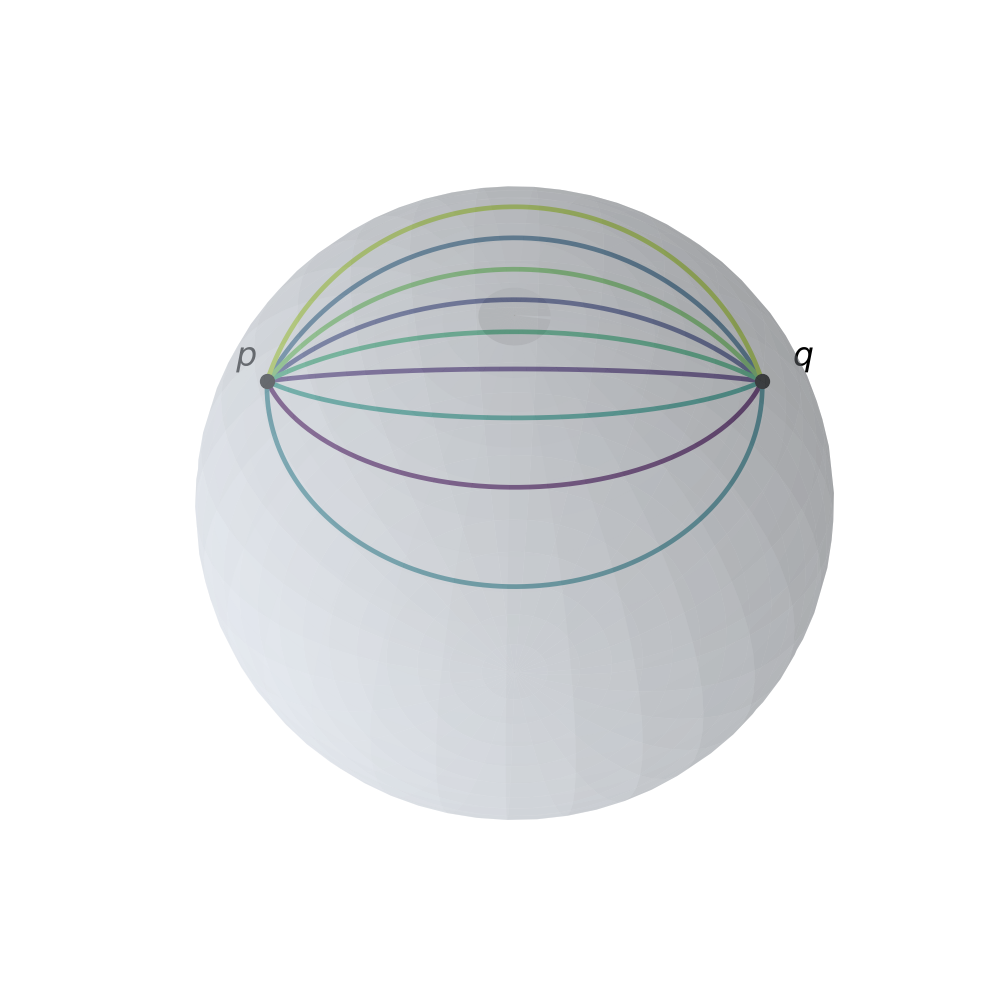
\includegraphics[width=0.48\textwidth]{fig_pencil.png}
\caption{Arcs of the pencil of circles through $p$ and $q$ on the sphere of radius $\tfrac12$. Distinct arcs meet only at $p$ and $q$, and together they sweep the sphere once.}
\label{fig:pencil}
\end{figure}

\begin{lemma}\label{lem:pencil}
The functions $f,k,\alpha$ are smooth, $\alpha$ is strictly increasing with $\alpha(\tau+2\pi)=\alpha(\tau)+\pi$, and
\[
\Bigl|\frac{d}{d\tau}f(\tau)^2\Bigr|\le 4\pi\,\frac{d\alpha}{d\tau}(\tau)\qquad\text{for all }\tau .
\]
\end{lemma}

\begin{proof}
Smoothness is clear from the explicit construction. Two distinct circles meet in at most two points, so the arcs $\Gamma_\tau$ have pairwise disjoint interiors; every point of $\Sp\setminus\{p,q\}$ lies on exactly one circle through $p$ and $q$, and on exactly one of its two arcs. Hence, as $\tau$ increases by $2\pi$, the arcs sweep $\Sp$ exactly once and monotonically, which gives the statements about $\alpha$.

Let $N_\tau$ be the unit normal of $\Gamma_\tau$ pointing to the side into which the arcs move as $\tau$ increases. The first variation of length for a family with fixed endpoints is
\[
f'(\tau)=-\int_{\Gamma_\tau}k_N\,\langle\partial_\tau\Gamma,N_\tau\rangle\,ds,\qquad \alpha'(\tau)=\int_{\Gamma_\tau}\langle\partial_\tau\Gamma,N_\tau\rangle\,ds,
\]
where $k_N$ is the geodesic curvature measured with respect to $N_\tau$; the tangential part of the variation contributes only boundary terms, which vanish because the endpoints are fixed. Since $k_N=\pm k(\tau)$ is constant along $\Gamma_\tau$, $|f'(\tau)|=|k(\tau)|\,\alpha'(\tau)$.

It remains to show $|k(\tau)|f(\tau)\le 2\pi$. If $C_\tau$ is a great circle, $k=0$. Otherwise let $D$ be the disc bounded by $C_\tau$ on the side towards which it curves. The Gauss--Bonnet formula for $D$ reads $|k|\,L(C_\tau)+4\Area(D)=2\pi$, so $|k|\,L(C_\tau)\le2\pi$, and $f(\tau)<L(C_\tau)$ since $\Gamma_\tau$ is a proper arc of $C_\tau$. Therefore $|(f^2)'|=2f|k|\alpha'\le4\pi\alpha'$.
\end{proof}

\subsection{Square-root growth along the fibres}

\begin{lemma}\label{lem:sqrt}
For every $V\in\SU$ and $B\in\RR$,
\[
\dinf\bigl(e^{i\sigma_3B}V\bigr)^2\ \le\ \dinf(V)^2+2\pi|B| .
\]
\end{lemma}

\begin{proof}
Suppose first $\Pi(V)=q\neq p$. By (F2) a minimizing horizontal curve from $1$ to $V$ projects onto an arc $\Gamma_{\tau_0}$ of the pencil, so $f(\tau_0)=\dinf(V)$. Let $W_\tau$ be the horizontal lift of $\Gamma_\tau$ starting at $1$. By Lemma~\ref{lem:holonomy}, $W_\tau(1)=e^{i\sigma_3c(\tau)}V$ with $c(\tau)=\pm2(\alpha(\tau)-\alpha(\tau_0))$, a fixed sign. By Lemma~\ref{lem:pencil}, $c$ is a strictly monotone bijection of $\RR$, so there is $\tau_1$ with $c(\tau_1)=B$, and $|\alpha(\tau_1)-\alpha(\tau_0)|=|B|/2$. Integrating the inequality of Lemma~\ref{lem:pencil} between $\tau_0$ and $\tau_1$,
\[
\dinf\bigl(e^{i\sigma_3B}V\bigr)^2\le f(\tau_1)^2\le f(\tau_0)^2+4\pi|\alpha(\tau_1)-\alpha(\tau_0)|=\dinf(V)^2+2\pi|B| .
\]
Suppose next $\Pi(V)=p$, that is $V=e^{i\sigma_3s}$. Let $g$ be the $2\pi$-periodic function equal to $t(2\pi-t)$ on $[0,2\pi]$. It is continuous, and $|g'|\le2\pi$ away from the multiples of $2\pi$, so $g$ is $2\pi$-Lipschitz on $\RR$. By (F1), $\dinf(e^{i\sigma_3t})^2=g(t)$, hence $\dinf(e^{i\sigma_3(s+B)})^2=g(s+B)\le g(s)+2\pi|B|$.
\end{proof}

At $V=1$ the lemma is the familiar square-root law $\dinf(e^{i\sigma_3B})\le\sqrt{2\pi|B|}$ of the ball--box theorem; its content is that the same constant works at every point, with the square of the distance in place of the distance.

\subsection{Conclusion of the proof}

\begin{proof}[Proof of Theorem~\ref{thm:A}]
Horizontal curves have the same length for every $\I$, so $d_\I\le\dinf$. Fix $U$, choose $B$ as in Proposition~\ref{prop:infconv}, and put $X=\dinf(e^{i\sigma_3B}U)$, so that $d_\I(U)^2=X^2+\I B^2$. Lemma~\ref{lem:sqrt}, applied to $V=e^{i\sigma_3B}U$ and the shift $-B$, gives $\dinf(U)^2\le X^2+2\pi|B|$. If $2\pi|B|\le\I B^2$ then $\dinf(U)\le d_\I(U)$. Otherwise, since $x\mapsto\sqrt{x+a}-\sqrt{x+b}$ decreases on $[0,\infty)$ when $a>b\ge0$,
\begin{align*}
\dinf(U)-d_\I(U)&\le\sqrt{X^2+2\pi|B|}-\sqrt{X^2+\I B^2}\le\sqrt{2\pi}\,t-\sqrt{\I}\,t^2\Big|_{t=\sqrt{|B|}}\\
&\le\max_{t\ge0}\bigl(\sqrt{2\pi}\,t-\sqrt{\I}\,t^2\bigr)=\frac{\pi}{2\sqrt{\I}} .
\end{align*}
For the lower bound take $U=e^{i\sigma_3z}$ with $z\in(0,\pi]$. The curve $e^{i\sigma_3tz}$, $t\in[0,1]$, has $h_3\equiv-z$ and length $\sqrt{\I}\,z$, so $d_\I(U)\le\sqrt{\I}z$, while $\dinf(U)=\sqrt{z(2\pi-z)}$ by (F1). Choose $z=\pi\bigl(1-\sqrt{\I/(\I+1)}\bigr)$. Then $2\pi z-z^2=\pi^2/(\I+1)$ and
\[
\dinf(U)-d_\I(U)\ \ge\ \frac{\pi}{\sqrt{\I+1}}-\sqrt{\I}\,\pi\Bigl(1-\sqrt{\tfrac{\I}{\I+1}}\Bigr)=\pi\bigl(\sqrt{\I+1}-\sqrt{\I}\bigr)=\frac{\pi}{\sqrt{\I}+\sqrt{\I+1}} .\qedhere
\]
\end{proof}

\begin{remark}
The point $e^{i\sigma_3z}$ used for the lower bound has $d_\I\le\sqrt{\I}\,z\approx\pi/(2\sqrt{\I})$, a curvature length from the identity, in agreement with the location of the largest discrepancy described in \cite{BFLS23}. In the normalization \eqref{eq:metric} the direct synthesis of $e^{i\sigma_3z}$ costs $\sqrt{\I}\,z$; the value $\I z$ printed in \cite{BFLS23} corresponds to measuring the penalty in units of $\sqrt{\I}$ and does not affect any conclusion there. The two bounds of Theorem~\ref{thm:A} differ by $O(\I^{-3/2})$. Whether the supremum equals $\pi/(\sqrt{\I}+\sqrt{\I+1})$ for every $\I$, that is, whether it is always attained on the fibre through the identity, is left open.
\end{remark}

\subsection{One-qubit states and the deformed Bloch sphere}

The complexity of a state $\psi$ relative to a reference state $\psi_0$ is the least complexity of a unitary carrying $\psi_0$ to $\psi$ \cite{BS19}:
\[
\delta_\I(\psi_0,\psi)=\min\{d_\I(U):U\psi_0=\psi\}.
\]

\begin{corollary}\label{cor:states}
For all states $\psi_0,\psi$ of one qubit and every $\I>0$, $0\le\delta_\infty(\psi_0,\psi)-\delta_\I(\psi_0,\psi)\le\pi/(2\sqrt{\I})$.
\end{corollary}

\begin{proof}
Both minima are over the same closed set of unitaries, on which $d_\I\le\dinf\le d_\I+\pi/(2\sqrt{\I})$ by Theorem~\ref{thm:A}.
\end{proof}

When $\psi_0$ is the north pole of the Bloch sphere, Brown and Susskind showed that $\delta_\I$ is the distance of the metric
\begin{equation}\label{eq:bloch}
4\,ds^2=d\theta^2+\frac{\I\sin^2\theta}{\I\cos^2\theta+\sin^2\theta}\,d\phi^2
\end{equation}
on the two-sphere \cite[equations~(3.9)--(3.10)]{BS19}. By Corollary~\ref{cor:states}, sending $\I\to\infty$ changes all its distances by less than $\pi/(2\sqrt{\I})$. The area behaves very differently.

\begin{proposition}\label{prop:area}
For $\I>1$ the area of \eqref{eq:bloch} equals
\[
\pi\sqrt{\frac{\I}{\I-1}}\;\arsinh\sqrt{\I-1}\ =\ \frac{\pi}{2}\log(4\I)+o(1)\qquad(\I\to\infty).
\]
\end{proposition}

\begin{proof}
The area element of \eqref{eq:bloch} is $\tfrac14\sqrt{\I}\sin\theta\,(\I\cos^2\theta+\sin^2\theta)^{-1/2}d\theta\,d\phi$. Integrating over $\phi$ and substituting $u=\cos\theta$,
\[
\Area=\frac{\pi}{2}\sqrt{\I}\int_{-1}^{1}\frac{du}{\sqrt{1+(\I-1)u^2}}=\frac{\pi\sqrt{\I}}{\sqrt{\I-1}}\arsinh\sqrt{\I-1}.
\]
Since $\arsinh x=\log\bigl(x+\sqrt{1+x^2}\bigr)=\log(2x)+O(x^{-2})$, the area is $\tfrac{\pi}{2}\log(4\I)+o(1)$.
\end{proof}

For $\I=1$ the formula, read as a limit, gives the area $\pi$ of the round Bloch sphere of radius $\tfrac12$. Proposition~\ref{prop:area} confirms the statement of \cite[Supplementary Information~3]{BFLS23} that the volume diverges logarithmically while distances move by a vanishing amount.

\section{Parallel parking}\label{sec:parking}

\subsection{The metric and the calibrating functions}

The configuration of the unicycle is its position $(y,z)$ in the plane, with $z$ the distance towards the curb, and its heading $\theta\in\RR/2\pi$, the rolling direction being $(\cos\theta,\sin\theta)$. Following \cite{BFLS23} we use
\begin{equation}\label{eq:se2}
ds^2=(\cos\theta\,dy+\sin\theta\,dz)^2+\I\,(\sin\theta\,dy-\cos\theta\,dz)^2+d\theta^2,\qquad 1\le\I<\infty,
\end{equation}
and for $\I=\infty$ the sub-Riemannian metric obtained by admitting only curves with $\sin\theta\,dy-\cos\theta\,dz=0$ (the unicycle cannot drift). In terms of the rolling speed $u$, the drift speed $v$ and the turning speed $w=\dot\theta$,
\[
\dot y=u\cos\theta+v\sin\theta,\qquad \dot z=u\sin\theta-v\cos\theta,\qquad ds^2=(u^2+\I v^2+w^2)\,dt^2 .
\]
The parking cost $C_\I(z)$ is the infimum of the lengths of curves from $(0,0,0)$ to $(0,z,0)$; the metric \eqref{eq:se2} is invariant under rigid motions of the plane, which is the left-invariance of \cite{BFLS23} in the group of motions of the plane, studied in the sub-Riemannian case by Sachkov \cite{Sac11}. Since $(\cos\theta\,dy+\sin\theta\,dz)^2+(\sin\theta\,dy-\cos\theta\,dz)^2=dy^2+dz^2$ and $\I\ge1$, every curve is at least as long as its projection to the plane, so $C_\I(z)\ge z$; for $\I=1$ drifting straight to the curb shows $C_1(z)=z$. From now on $\I>1$.

For a function $\varphi(y,z,\theta)$ and a curve of unit speed, Cauchy--Schwarz gives $|\dot\varphi|\le\|d\varphi\|$, where for $d\varphi=a\,dy+b\,dz+c\,d\theta$
\[
\|d\varphi\|^2=(a\cos\theta+b\sin\theta)^2+\I^{-1}(a\sin\theta-b\cos\theta)^2+c^2,
\]
with $\I^{-1}=0$ when $\I=\infty$. If $\|d\varphi\|\le1$ everywhere, every curve from $P$ to $Q$ has length at least $|\varphi(Q)-\varphi(P)|$.

\begin{lemma}\label{lem:calib}
Let $\kappa=\sqrt{1-\I^{-1}}$, $\beta(\theta)=\kappa(1-\sin\theta)$ and $\tilde\beta(\theta)=\kappa(1+\sin\theta)$. Each of the four functions $z\pm\beta(\theta)$, $z\pm\tilde\beta(\theta)$ has $\|d\varphi\|=1$ at every point.
\end{lemma}

\begin{proof}
Here $a=0$, $b=1$ and $c=\pm\kappa\cos\theta$, so $\|d\varphi\|^2=\sin^2\theta+\I^{-1}\cos^2\theta+(1-\I^{-1})\cos^2\theta=1$.
\end{proof}

\subsection{The lower bound}

Let $\gamma$ be a curve of length $L$ from $(0,0,0)$ to $(0,z,0)$, and let $M=\max_\gamma|\sin\theta|$, attained at a point $m=(y_m,z_m,\theta_m)$. Suppose $\sin\theta_m=M$. Using $\varphi_-=z-\beta$ on the part of $\gamma$ before $m$ and $\varphi_+=z+\beta$ on the part after $m$,
\[
L\ \ge\ \bigl[z_m-\kappa(1-M)+\kappa\bigr]+\bigl[z+\kappa-z_m-\kappa(1-M)\bigr]=z+2\kappa M .
\]
If $\sin\theta_m=-M$, the same computation with $z\mp\tilde\beta$ gives the same bound. On the other hand $|\dot z|\le\|dz\|=(\sin^2\theta+\I^{-1}\cos^2\theta)^{1/2}\le(M^2+\I^{-1}(1-M^2))^{1/2}$ along $\gamma$, so
\[
L\ \ge\ z\,r(M),\qquad r(M)=\bigl(M^2+\I^{-1}(1-M^2)\bigr)^{-1/2}.
\]
Write $\varepsilon=1-M$. For $\I<\infty$, $r^2-1=\kappa^2(1-M^2)/(1-\kappa^2(1-M^2))\ge\kappa^2\varepsilon$ and $1\le r\le\sqrt{\I}$, so $r-1\ge\kappa^2\varepsilon/(1+\sqrt{\I})$; for $\I=\infty$, $r-1=\varepsilon/(1-\varepsilon)\ge\varepsilon$. In both cases $L-z\ge\max\{a(1-\varepsilon),\,b\varepsilon\}\ge ab/(a+b)$ with $a=2\kappa$ and $b=z\kappa^2/(1+\sqrt{\I})$, respectively $a=2$, $b=z$. This is the lower bound of Theorem~\ref{thm:B}.

\subsection{The upper bound}

The construction follows the gradient lines of the calibrating functions. On a unit-speed curve, $\dot\varphi_-=1$ for $\varphi_-=z-\beta$ forces
\begin{equation}\label{eq:grad}
u=\sin\theta,\qquad v=-\I^{-1}\cos\theta,\qquad w=\kappa\cos\theta,
\end{equation}
and then $\dot z=\sin^2\theta+\I^{-1}\cos^2\theta$ and $\dot y=\kappa^2\sin\theta\cos\theta$. For $\I=\infty$ the drift vanishes, as it must. Fix $\varepsilon\in(0,\pi/2)$ and put $\theta_1=\pi/2-\varepsilon$. The manoeuvre has five stages (Figure~\ref{fig:parking}).

\begin{enumerate}
\item Follow \eqref{eq:grad} from heading $0$ to heading $\theta_1$. Since $\varphi_-$ increases at unit rate, the cost equals the increase of $z$ plus $\beta(0)-\beta(\theta_1)=\kappa\cos\varepsilon$. With $ds=d\theta/(\kappa\cos\theta)$, the gain in $z$ is
\[
Z_1=\int_0^{\theta_1}\frac{\sin^2\theta+\I^{-1}\cos^2\theta}{\kappa\cos\theta}\,d\theta\le\frac1\kappa\log\frac{1+\cos\varepsilon}{\sin\varepsilon}\le\frac1\kappa\log\frac{\pi}{\varepsilon},
\]
and the gain in $y$ is $\kappa\int_0^{\theta_1}\sin\theta\,d\theta=\kappa(1-\sin\varepsilon)$.
\item Turn on the spot from $\theta_1$ to $\pi/2$, at cost $\varepsilon$.
\item With $Y=2\kappa(1-\sin\varepsilon)$, $m=z-2Z_1>0$ and $\delta=\arctan(Y/m)$, turn to heading $\pi/2+\delta$, roll a length $\sqrt{m^2+Y^2}$, and turn back to $\pi/2$. This moves the unicycle by $(-Y,m)$ at cost $\sqrt{m^2+Y^2}+2\delta\le m+(Y^2/2+2Y)/m$.
\item Turn on the spot from $\pi/2$ to $\theta_1$, at cost $\varepsilon$.
\item Follow $u=\sin\theta$, $v=-\I^{-1}\cos\theta$, $w=-\kappa\cos\theta$ from $\theta_1$ down to $0$. This is the gradient line of $\varphi_+=z+\beta$, so again the cost is the gain in $z$, equal to $Z_1$, plus $\kappa\cos\varepsilon$, and the gain in $y$ is again $\kappa(1-\sin\varepsilon)$.
\end{enumerate}

The unicycle ends at $(0,z,0)$, and the total cost is at most
\[
z+2\kappa\cos\varepsilon+2\varepsilon+\frac{2\kappa^2+4\kappa}{m}.
\]
Take $\varepsilon=1/z$. If $z\ge2$ and $z\ge(4/\kappa)\log(\pi z)$, then $2Z_1\le(2/\kappa)\log(\pi z)\le z/2$, so $m\ge z/2$ and the cost is at most $z+2\kappa+(2+8\kappa+4\kappa^2)/z$. This completes the proof of Theorem~\ref{thm:B}. \qed

\begin{figure}[H]
\centering
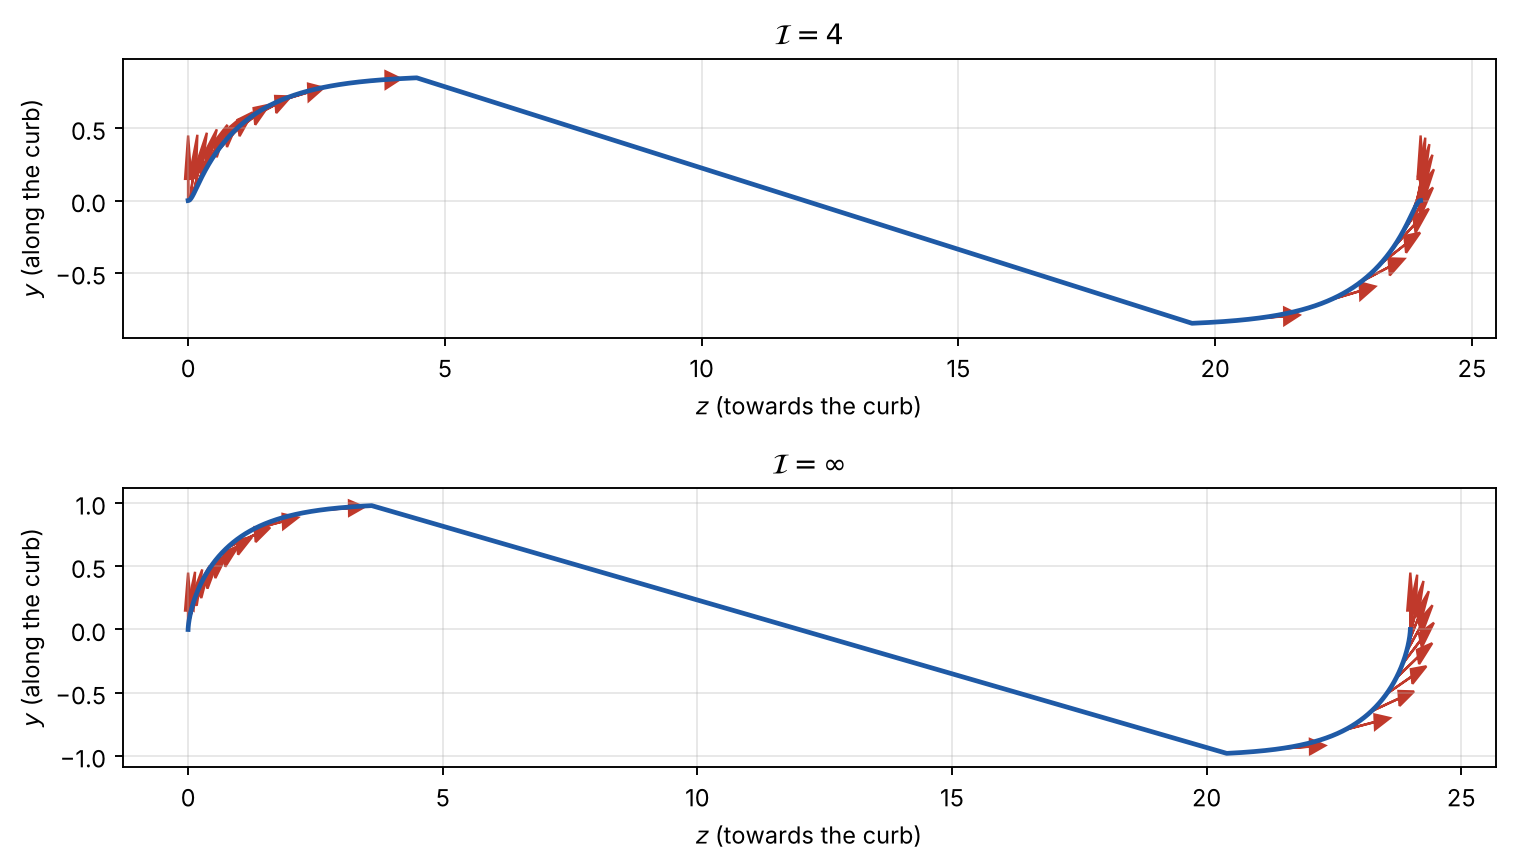
\includegraphics[width=0.92\textwidth]{fig_parking.png}
\caption{The manoeuvre of the upper bound for $z=24$, for $\I=4$ (top) and $\I=\infty$ (bottom). Arrows show the heading. The unicycle turns while it rolls, drifts back across the long middle stage, and turns back while it rolls into the parking spot.}
\label{fig:parking}
\end{figure}

\subsection{The manoeuvre turn, roll, turn}

The upper bound $C_\I(z)\le z+\pi$ of \cite{BFLS23}, obtained by turning through a right angle, rolling to the curb and turning back, holds for every $z$. Optimizing over the turning angle $\phi$, with the middle stage replaced by the straight motion that combines rolling and drifting, costs $2\phi+z\,n(\phi)$, $n(\phi)=(\sin^2\phi+\I\cos^2\phi)^{1/2}$. With $c=\cos\phi$ one has $2\phi\ge\pi-\pi c$ and $n(\phi)\ge1+(\I-1)c^2/(2\sqrt{\I})$, so
\[
2\phi+z\,n(\phi)-z\ \ge\ \pi-\pi c+\frac{z(\I-1)c^2}{2\sqrt{\I}}\ \ge\ \pi-\frac{\pi^2\sqrt{\I}}{2(\I-1)z}.
\]
Hence the optimized turn--roll--turn manoeuvre costs $z+\pi+o(1)$ for every $\I>1$, strictly more than the true cost $z+2\kappa+O(1/z)$, since $2\kappa<2<\pi$. The constant $2\sqrt{1-\I^{-1}}$ of \eqref{eq:BFLS6} is correct, but it is reached only by turning and rolling at the same time, as in \eqref{eq:grad}. For $\I=1$ the two constants are $0$ and $\pi$, and the optimum is not to turn at all.

\section{Discussion}\label{sec:discussion}

Theorems~\ref{thm:A} and~\ref{thm:B} make the two low-dimensional examples of \cite{BFLS23} rigorous. On the Berger sphere the volume tends to infinity with $\I$, while by Theorem~\ref{thm:A} no distance moves by more than $\pi/(2\sqrt{\I})$. For the unicycle the short-distance geometry depends strongly on $\I$, but by Theorem~\ref{thm:B} the long-distance growth has slope $1$ for every $\I\ge1$, and $\I$ enters only through the additive constant $2\sqrt{1-\I^{-1}}$, a smooth function of $\I^{-1}$ on $[0,1]$. In the language of \cite{BFLS23} the penalty factor is an irrelevant deformation, and Theorem~\ref{thm:B} identifies its effect exactly. The two mechanisms behind the proofs, a quadratic infimal convolution along a central direction and calibration by functions with unit differential, are not special to these groups, and it would be interesting to know how far they reach towards the high-dimensional conjectures of \cite{BFLS23}.

\section*{Acknowledgements}

The author acknowledges that the questions treated here were formulated by Brown, Freedman, Lin and Susskind \cite{BFLS23}, building on the single-qubit analysis of Brown and Susskind \cite{BS19} and on the complexity geometry of Nielsen, Dowling, Gu and Doherty \cite{NDGD06}; the sub-Riemannian facts used in Section~\ref{sec:berger} are due to Boscain and Rossi \cite{BR08}. The related negative-curvature picture of complexity is that of Brown, Susskind and Zhao \cite{BSZ17}. Earlier work of the author on hyperbolic groups, hypercomplex structures and toric geometry appears in \cite{Bha22a,Bha22b,BSN26}.

\section*{Declarations}

\noindent\textbf{Data availability.} No data were generated. The \LaTeX\ source and the script that draws the figures are archived at \href{https://doi.org/\zenodoCodeDOI}{doi:\zenodoCodeDOI}.

\smallskip\noindent\textbf{Funding.} The author received no funding for this work.

\smallskip\noindent\textbf{Conflict of interest.} The author declares no conflict of interest.

\smallskip\noindent\textbf{Ethics statement.} This work involves no human or animal subjects.

\begin{thebibliography}{99}

\bibitem{Bha22a} D.~Bhattacharjee, Non-commutativity over canonical suspension $\eta$ for genus $g\ge1$ in hypercomplex structures for potential $\rho\phi$, \emph{Asian Res. J. Math.} \textbf{18} (2022), no.~11, 332--341. doi:10.9734/arjom/2022/v18i11607.

\bibitem{Bha22b} D.~Bhattacharjee, Establishing equivariant class $[O]$ for hyperbolic groups, \emph{Asian Res. J. Math.} \textbf{18} (2022), no.~11, 362--369. doi:10.9734/arjom/2022/v18i11615.

\bibitem{BSN26} D.~Bhattacharjee, S.~Singha Roy and P.~Nandi, Hodge--toric geometry beyond CY20, \emph{Int. J. Prof. Stud.} \textbf{21} (2026), no.~1. doi:10.37648/ijps.v21i01.019.

\bibitem{BR08} U.~Boscain and F.~Rossi, Invariant Carnot--Caratheodory metrics on $S^3$, $SO(3)$, $SL(2)$, and lens spaces, \emph{SIAM J. Control Optim.} \textbf{47} (2008), no.~4, 1851--1878. doi:10.1137/070703727.

\bibitem{BFLS23} A.~R.~Brown, M.~H.~Freedman, H.~W.~Lin and L.~Susskind, Universality in long-distance geometry and quantum complexity, \emph{Nature} \textbf{622} (2023), 58--62. doi:10.1038/s41586-023-06460-3.

\bibitem{BS19} A.~R.~Brown and L.~Susskind, Complexity geometry of a single qubit, \emph{Phys. Rev. D} \textbf{100} (2019), 046020. doi:10.1103/PhysRevD.100.046020.

\bibitem{BSZ17} A.~R.~Brown, L.~Susskind and Y.~Zhao, Quantum complexity and negative curvature, \emph{Phys. Rev. D} \textbf{95} (2017), 045010. doi:10.1103/PhysRevD.95.045010.

\bibitem{Mon02} R.~Montgomery, \emph{A Tour of Subriemannian Geometries, Their Geodesics and Applications}, Math. Surveys Monogr. \textbf{91}, American Mathematical Society, Providence, RI, 2002. doi:10.1090/surv/091.

\bibitem{NDGD06} M.~A.~Nielsen, M.~R.~Dowling, M.~Gu and A.~C.~Doherty, Quantum computation as geometry, \emph{Science} \textbf{311} (2006), 1133--1135. doi:10.1126/science.1121541.

\bibitem{Pod18} A.~V.~Podobryaev, Diameter of the Berger sphere, \emph{Math. Notes} \textbf{103} (2018), no.~5--6, 846--851. doi:10.1134/S0001434618050188.

\bibitem{Sac11} Yu.~L.~Sachkov, Cut locus and optimal synthesis in the sub-Riemannian problem on the group of motions of a plane, \emph{ESAIM Control Optim. Calc. Var.} \textbf{17} (2011), no.~2, 293--321. doi:10.1051/cocv/2010005.

\end{thebibliography}

\end{document}
